\section{Powerfit protocol}
\label{app:powerfitProtocol}%a160
Protocol designed to automatically fit atomic structures to electron density maps in \scipion by using $PowerFit$ (\citep{vanzundert2016}), application that performs a rigid body search based on cross-correlation between atomic structure and electron density map. You can follow additional instructions to run $PowerFit$ in \url{http://www.bonvinlab.org/education/powerfit/}.\\

   
 \begin{itemize}
  \item \scipion menu:\\
   \ttt{Protocols SPA -> Model building} (\ffigure{fig:app_protocol_powerfit_1} (A))\\
  
  \item Protocol form parameters (\ffigure{fig:app_protocol_powerfit_1} (B)):\\
  
    \begin{figure}[H]
     \centering 
     \captionsetup{width=.7\linewidth} 
     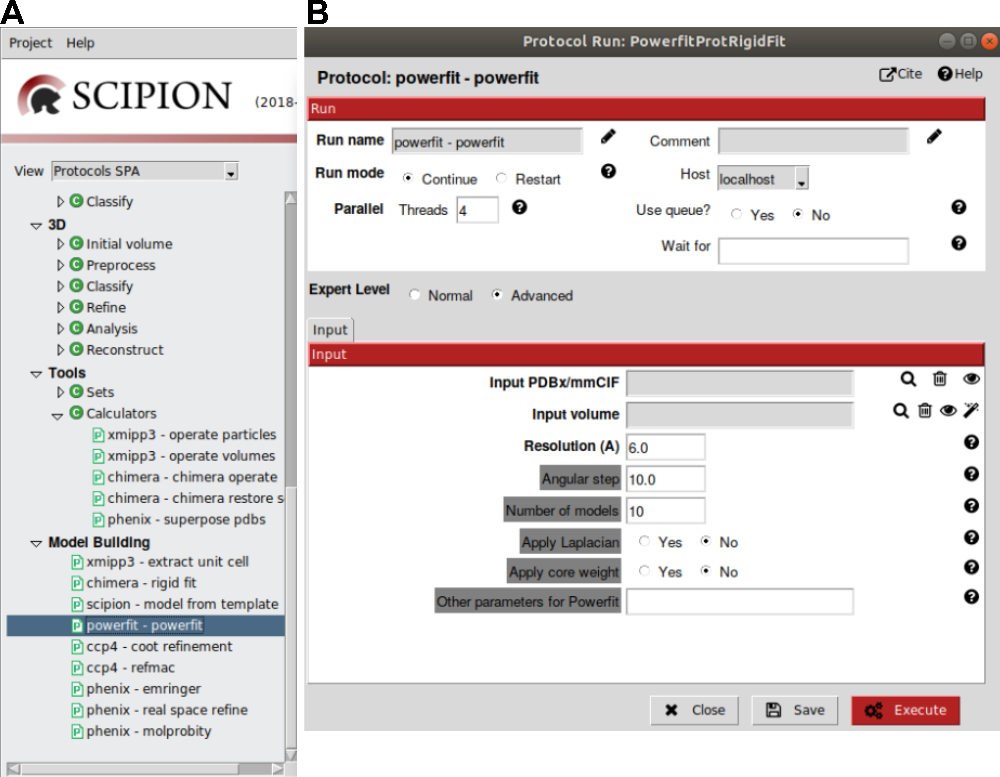
\includegraphics[width=0.90\textwidth]{Images_appendix/Fig113.pdf}
     \caption{Protocol \scommand{powerfit}. A: Protocol location in \scipion menu. B: Protocol form.}
     \label{fig:app_protocol_powerfit_1}
    \end{figure}

    \begin{itemize}
     \item \ttt{Input atomic structure to fit}: Atomic structure previously downloaded or generated in \scipion to be fitted to an electron density map.\\
     \item \ttt{Input volume}: Electron density map previously downloaded or generated in \scipion to fit the atomic structure.\\ %OJO: Hay un wizard que no funciona\\
     \item \ttt{Resolution (\AA)}: Electron density map resolution.\\
     \item \ttt{Angular step}: Advanced parameter to indicate rotational sampling interval (degrees). 10º is the default value. Lower values usually generate better fits because they allow more subtle searches in the 3D space. However, the process gets computationally more expensive. So, this parameter value should be carefully selected considering the whole size of the molecule. An estimation of $PowerFit$ runtime can be checked here: \url{http://milou.science.uu.nl/cgi/services/POWERFIT/powerfit/}.\\
     \item \ttt{Number of models}: Advanced parameter to select the maximum number of fits generated, 10 by default. To avoid structure redundancy, a lower number of best fit structures than indicated might be shown by $PowerFit$.\\
     \item \ttt{Apply Laplacian}: Advanced parameter to apply a Laplacian pre-filter to the electron density map to enhance its edges and increase cross-correlation scores between atomic structure and electron density map. Parameter set to "No" by default.\\
     \item \ttt{Apply core weight}: Advanced parameter of local cross-correlation score, designed to bias the weight of electron density toward the core of the map, thus minimizing the effect of overlapping among neighboring subunits. Parameter set to "No" by default.\\
     \item \ttt{Other parameters for $Powerfit$}: Advanced parameter to include, for instance, the number of CPU available or if GPU is going to be used for computation.\\
    \end{itemize}

  \item Protocol execution:\\
  
  Adding specific protocol label is recommended in \ttt{Run name} section, at the form top. To add the label, open the protocol form, press the pencil symbol at the right side of \ttt{Run name} box, complete the label in the new opened window, press OK, and finally, close the protocol. This label will be shown in the output summary content (see below). If you want to run again this protocol, do not forget to set to \ttt{Restart} the \ttt{Run mode}.\\
  Press the \ttt{Execute} red button at the form bottom.\\
  
  \item Visualization of protocol results:\\
  
  After executing the protocol, press \ttt{Analyze Results} and a small window will be opened (\ffigure{fig:app_protocol_powerfit_2}). This window allows selecting between visualize fitting quality scores and the fitting itself in \chimera for each non-redundant fit generated by $PowerFit$. The number inside \ttt{Model to visualize} box allows to select one specific fit.\\
  
  \begin{figure}[H]
    \centering 
    \captionsetup{width=.7\linewidth} 
    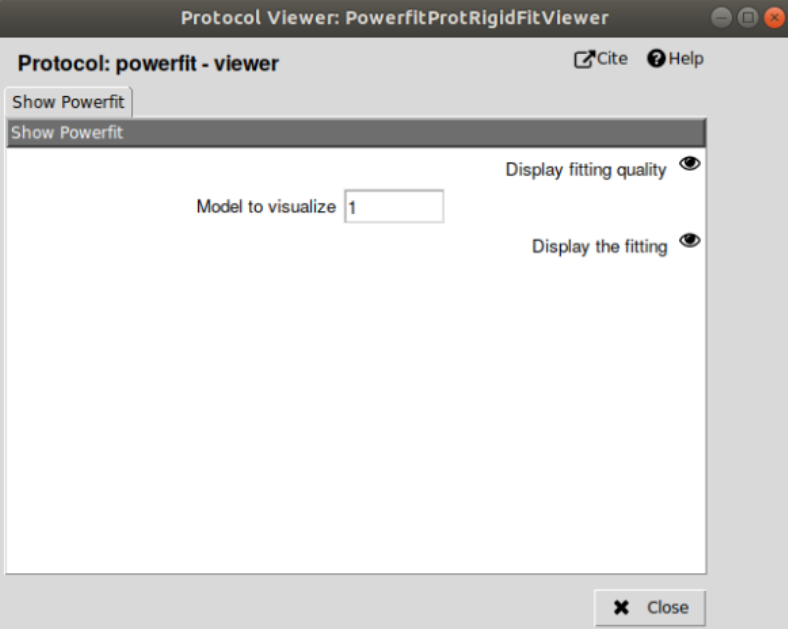
\includegraphics[width=0.60\textwidth]{Images_appendix/Fig114.pdf}
    \caption{Protocol \scommand{powerfit}. Menu to visualize $PowerFit$ results.}
    \label{fig:app_protocol_powerfit_2}
   \end{figure}
   
   \begin{itemize}
   
    \item \ttt{Display fitting quality}:\\
    
    When this option is selected, a five-column table opens (\ffigure{fig:app_protocol_powerfit_3}). First and second columns of this table contains rank and file name of best fits generated by $PowerFit$. Cross correlation score between atomic structure and electron density map, Fisher Z-score, and the number of standard deviations are values included in \ttt{\_powerfit\_cc}, \ttt{\_powerfit\_Fish\_z}, and \ttt{\_powerfit\_rel\_z} columns, respectively.\\
   
     \begin{figure}[H]
      \centering 
      \captionsetup{width=.7\linewidth} 
      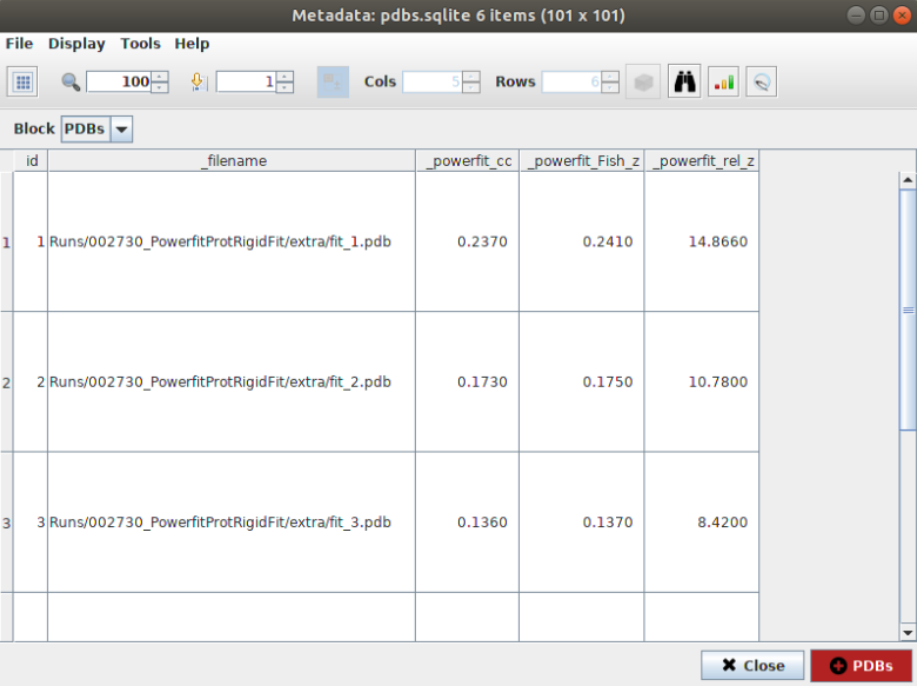
\includegraphics[width=0.70\textwidth]{Images_appendix/Fig115.pdf}
      \caption{Protocol \scommand{powerfit}. Fitting quality scores of $PowerFit$ results.}
      \label{fig:app_protocol_powerfit_3}
     \end{figure}
   
    \item \ttt{Display the fitting}:\\
   
    After executing the protocol, press \ttt{Analyze Results} and \chimera graphics window will be opened by default. Atomic structures and volumes are referred to the origin of coordinates in \chimera. To show the relative position of atomic structure and electron density volume, the three coordinate axes are represented; X axis (red), Y axis (yellow), and Z axis (blue) (\ffigure{fig:app_protocol_volume_3}). Coordinate axes, volume, and each atomic structure are model numbers \ttt{\#0}, \ttt{\#1}, and \ttt{\#3}, respectively, in \chimera \ttt{Model Panel} (\ffigure{fig:app_protocol_powerfit_3}). Model number \ttt{\#2} corresponds to \ttt{lcc.mrc} volume, i.e., a cross-correlation density map that shows the highest cross-correlation found in each grid position, indicating the most likely location of the center of mass of the atomic structure.\\

   \end{itemize}
   
  \item Summary content:\\
  
   \begin{itemize}
     \item Protocol output (below \scipion framework):\\ \ttt{powerfit - powerfit -> ouputPDBs}; \ttt{SetOfPDBs (\ttt{\#n} items)}.\\ n items indicates the number of non-redundant structures best fitted to the electron density map, found by $PowerFit$.\\
     \item \ttt{SUMMARY} box:\\Angular step: 10.000000\\
    \end{itemize}
  
 \end{itemize}
